
\chapter{协议实现}

\section{Pipelining 实现}

本周的实现较为简单。由于在 Lab2 中我们实现了缓冲区的自动化更新、防溢出。可以支持任意大小的文件传入。所以本周的任务中,我们只需要关注如何将收到的信息拆分为单个单个的报文。然后处理之即可。

我们的实现方式,是通过函数 strstr() 获得拆分每个报文。 strstr(str,dest) 函数得到 dest 在 str 第一次出现的地址。于是就能通过 strstr() 得到报文结束前 " \textbackslash r\textbackslash n\textbackslash r\textbackslash n "的位置。然后通过简单的字符串处理,就能开始处理单个报文了。部分代码如图\ref{fig:liso_server_pipelining}。

\begin{figure}[htbp!]
    \centering
    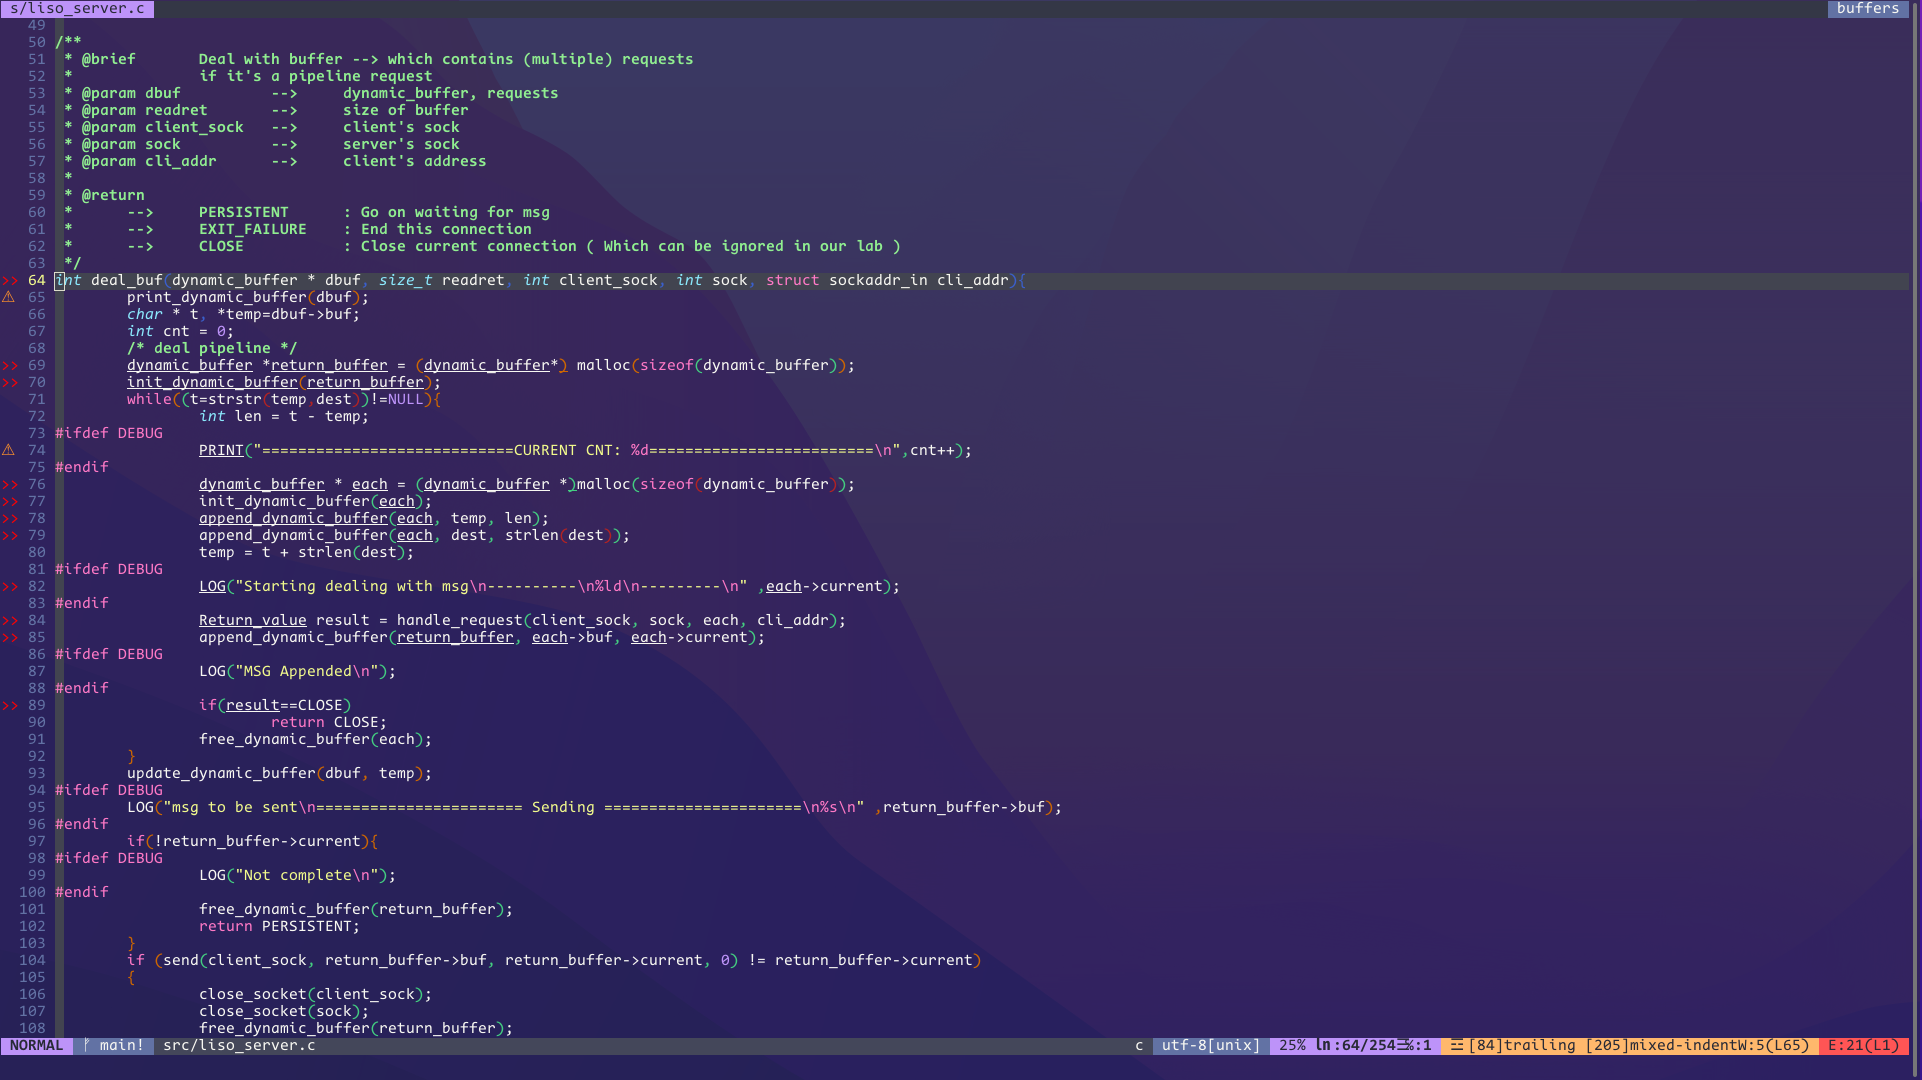
\includegraphics[width=6in]{liso_server_pipelining.png}
    \caption{Liso Server Pipelining}\label{fig:liso_server_pipelining}
\end{figure}



